\newpage
\section{User Functionalities}
\subsection{Registration}
\par \qquad To register the user have to open the "Main page".
\begin{figure}[tbh]
  \begin{center}
    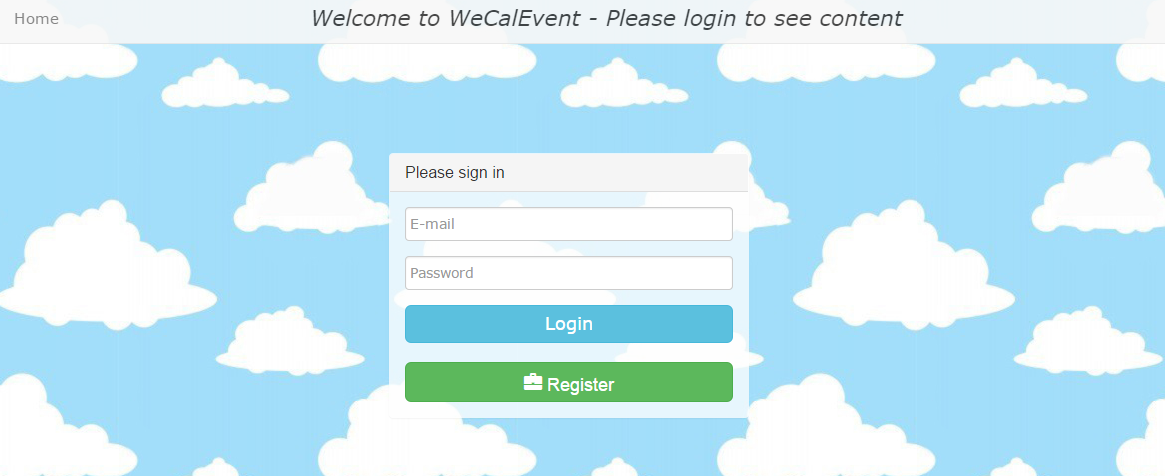
\includegraphics[width=100mm]{mainp}
  \end{center}
\end{figure}

\par After clicking on "Register" button the user will be redirected to the "Register page":
\begin{figure}[tbh]
  \begin{center}
    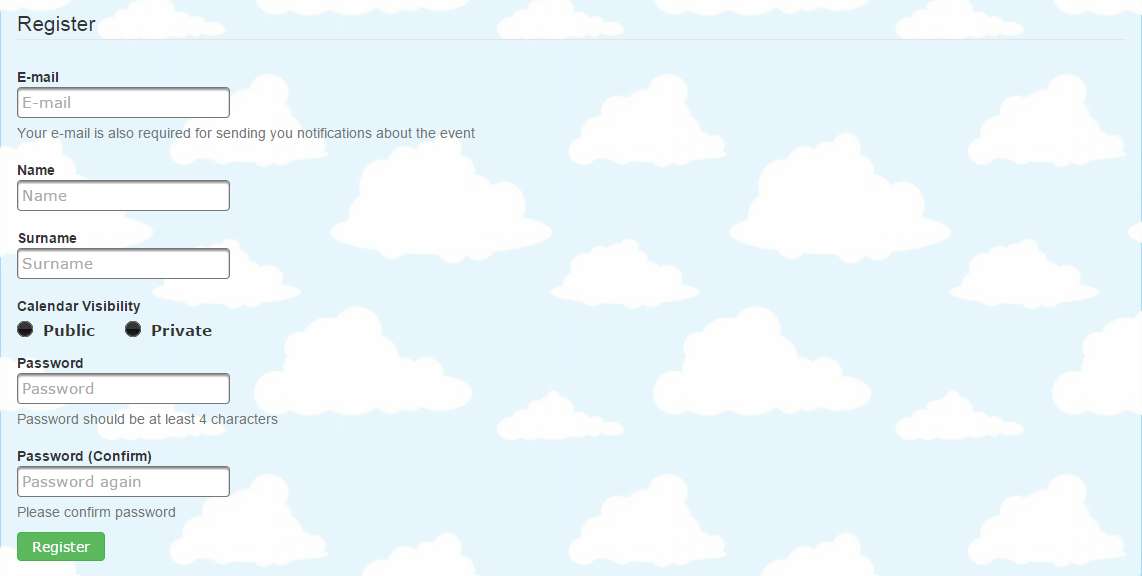
\includegraphics[width=100mm]{regp}
  \end{center}
\end{figure}

\par If all fields are filled in right the user will be registered after pressing "Register" button.
\par In case if not all fields are filled in, below notifications will appear:
        \begin{figure}[tbh]
         \begin{center}
          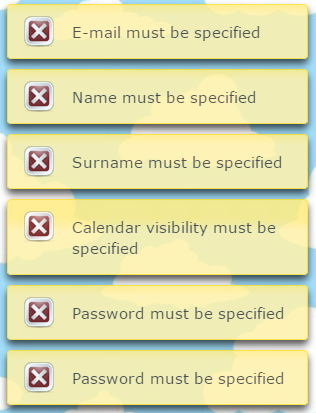
\includegraphics[width=50mm]{reger1}
         \end{center}
        \end{figure}

\newpage
\subsection{Login}
\par \qquad After the "Main page" was opened the user has to type her/his e-mail and password in the form shown below
\begin{figure}[tbh]
  \begin{center}
    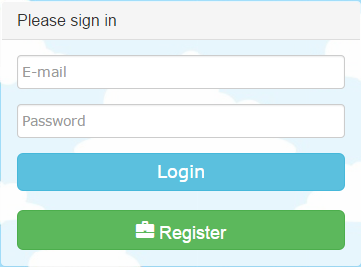
\includegraphics[width=50mm]{login}
  \end{center}
\end{figure}

\par Then the user has to click on "Login" button and if all fields are filled in right she/he will be logged in and redirected to the "Home page":
\begin{figure}[tbh]
  \begin{center}
    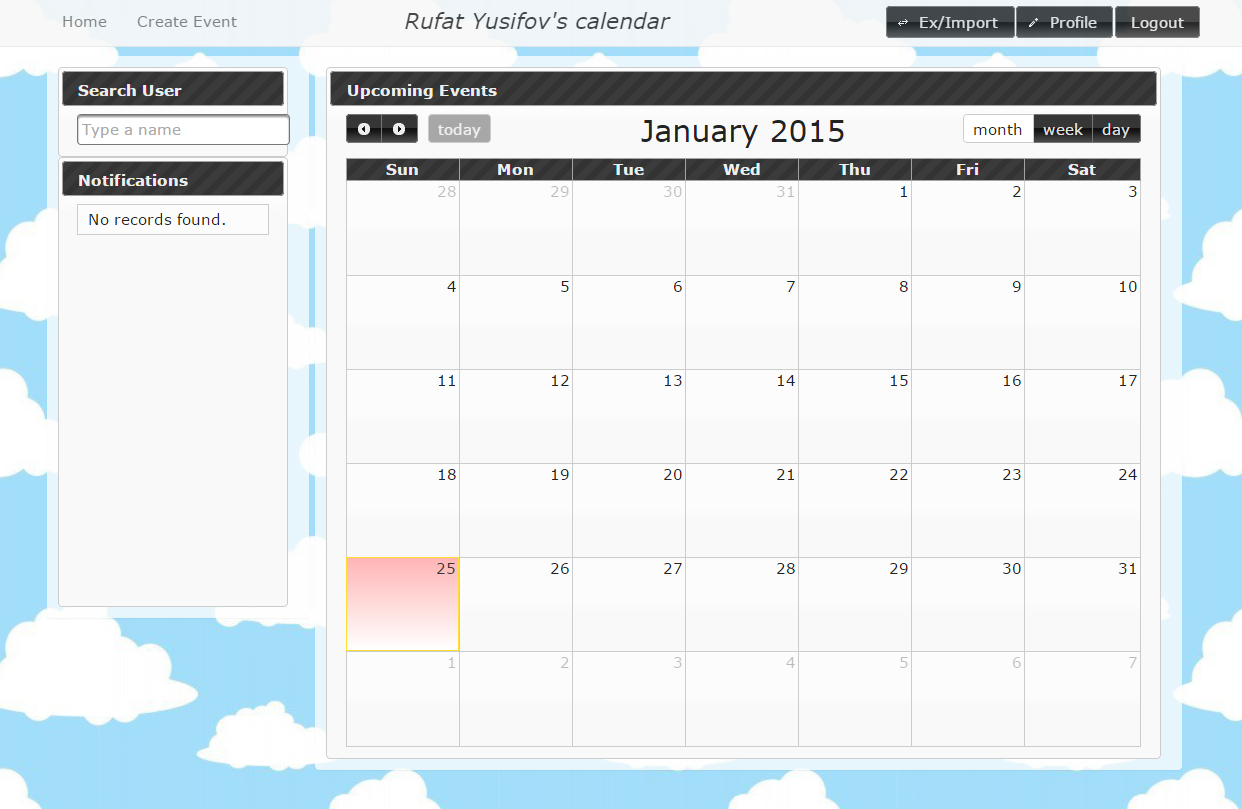
\includegraphics[width=120mm]{homep}
  \end{center}
\end{figure}

\par In case some of the fields were filled in wrong, below notification will appear:
\begin{figure}[tbh]
  \begin{center}
    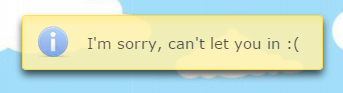
\includegraphics[width=50mm]{erlog}
  \end{center}
\end{figure}

\newpage
\subsection{Update profile}
\par \qquad To change her/his profile information the user should click on "Profile" button. After that the user will be redirected to the "Update profile page":
\begin{figure}[tbh]
  \begin{center}
    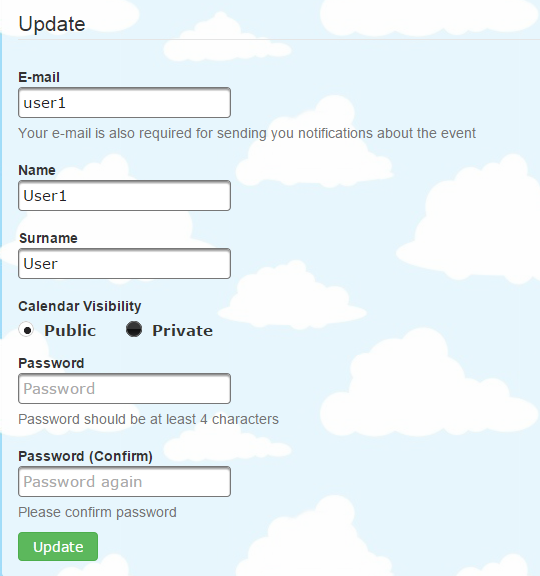
\includegraphics[width=50mm]{updatepr}
  \end{center}
\end{figure}

\par If all fields were filled in right the profile will be updated and the user will be redirected to the "Home page".
\par In case if some fields were not field in, appropriate notification will appear.

\subsection{Create an event}
\par \qquad To create an event the user has to click on the "Create Event" button and she/he will be redirected to the "Event creation" page:
\begin{figure}[tbh]
  \begin{center}
    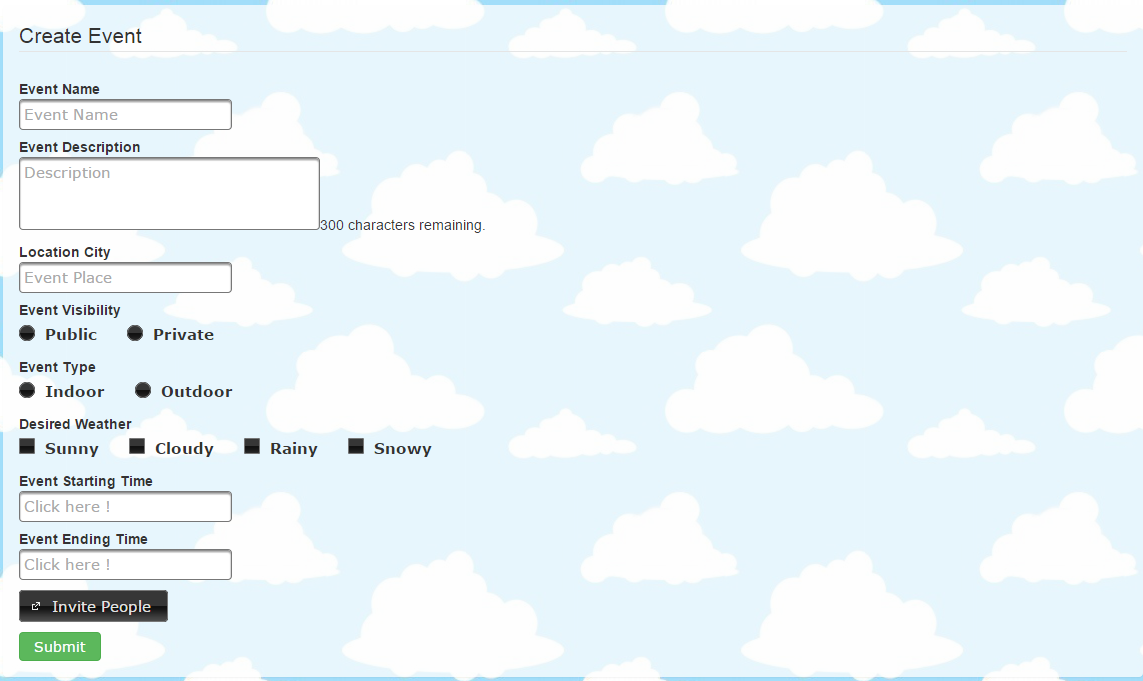
\includegraphics[width=100mm]{crevent}
  \end{center}
\end{figure}

\newpage
\par In case not all fields were filled in, below notifications will appear
 \begin{figure}[tbh]
  \begin{center}
    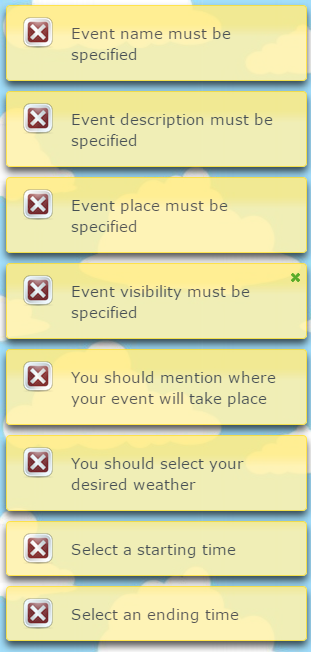
\includegraphics[width=40mm]{creventer1}
  \end{center}
\end{figure}

\subsection{Update an event}
\par \qquad To update an event the user has to choose an event she/he created in her/his calendar view.
\par After clicking on this event "View event" page will open:
  \begin{figure}[tbh]
  \begin{center}
    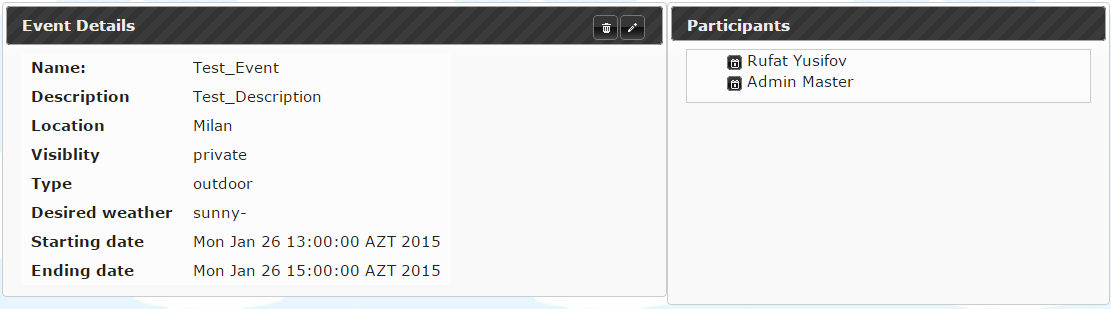
\includegraphics[width=150mm]{viewev}
  \end{center}
\end{figure}

\newpage
\par After clicking on "Update event" button the user will be redirected to the "Update event" page:
  \begin{figure}[tbh]
  \begin{center}
    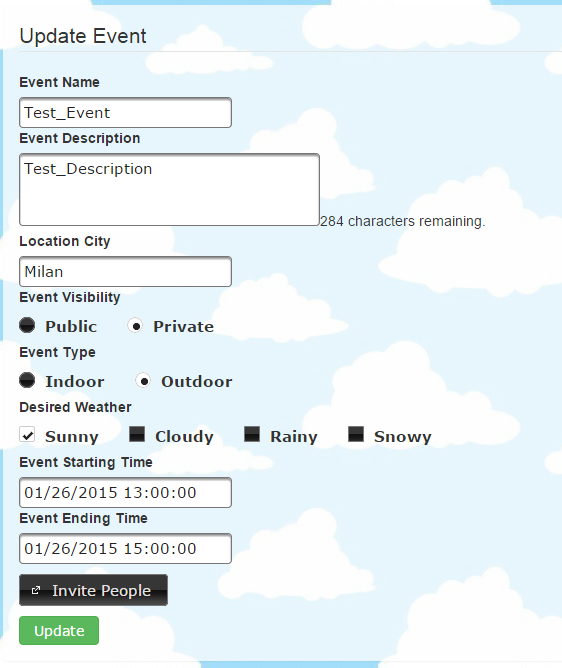
\includegraphics[width=100mm]{upevent}
  \end{center}
\end{figure}

\par To update the event the user has to click on "Update" button. If all fields were filled in right the event will be updated.
\par In case if some fields were not filled in or were filled in wrong an appropriate notification will appear.

\subsection{Delete an event}
\par \qquad To delete the event she/he created, the user has to click on it in her/his calendar view. After this the user will be redirected to the "View event" page. To delete an event the user should click on the "Delete" button.

\newpage
\subsection{Answer event invitation}
\par \qquad If the user was invited to an event she/he will receive an invitation notification:
  \begin{figure}[tbh]
  \begin{center}
    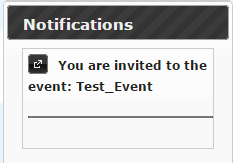
\includegraphics[width=30mm]{invnot}
  \end{center}
\end{figure} 

\par To answer the invitation the user has to click on this notification. Then the event information window will open:
  \begin{figure}[tbh]
  \begin{center}
    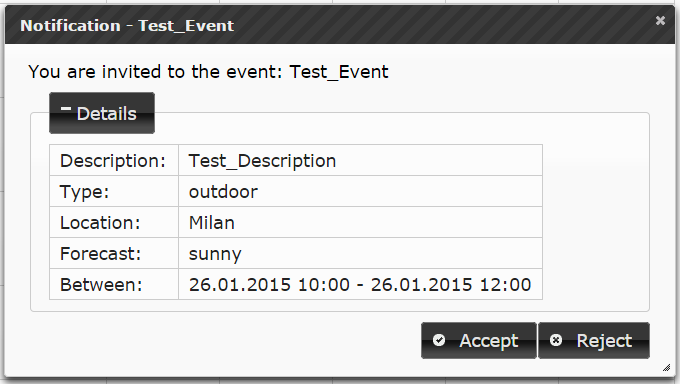
\includegraphics[width=100mm]{invit}
  \end{center}
\end{figure}

\par To accept (decline) the invitation the user should click on "Accept" ("Decline") button.

\subsection{Search users}
\par \qquad To search for another user the user should type the name in "Search User" field on "Home page".

\newpage
\subsection{Import/Export Calendar}
\par \qquad To Import/Export calendar the user has to click on "Ex/Import" button on "Home page". The the user will be redirected to the "Export/Import" page:
   \begin{figure}[tbh]
  \begin{center}
    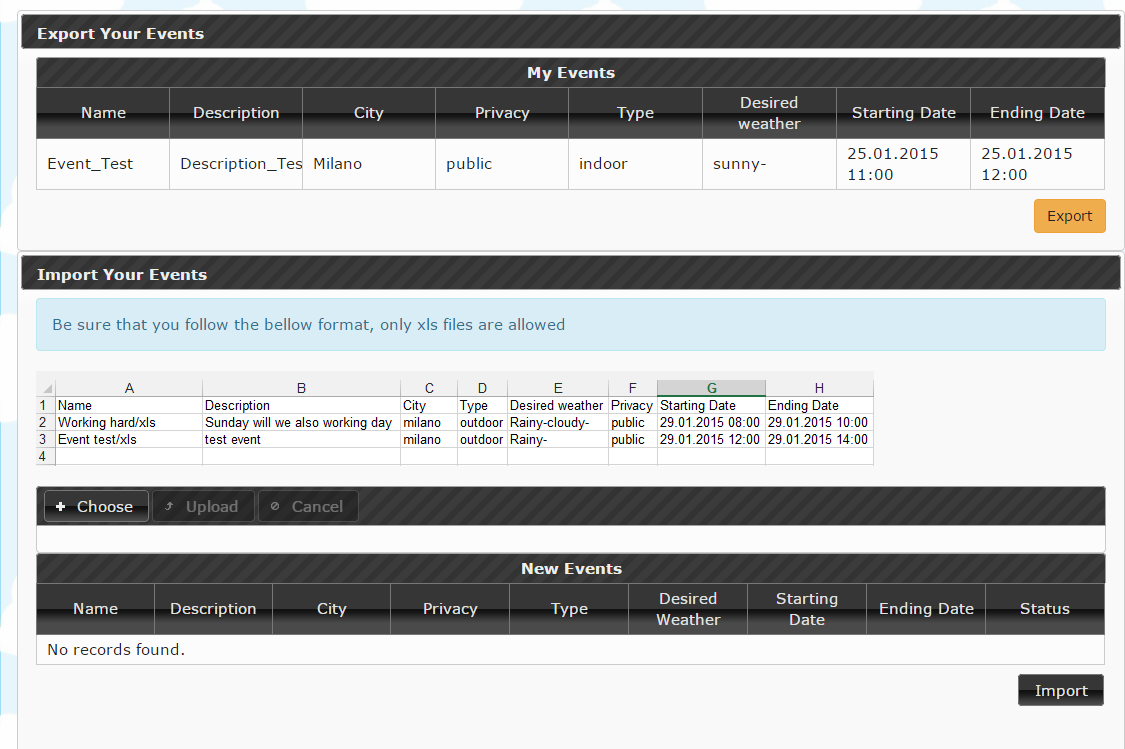
\includegraphics[width=100mm]{eximpo}
  \end{center}
\end{figure}

\par To export calendar the user should click on "Export" button.
\par To import calendar the user has to click on "Choose" button. After choosing the needed calendar the user should click on "Upload" button. If all fields are filled in an appropriate way, the calendar will be uploaded. TO import it the user has to click on "Import" button. 
\par In case if uploaded file has wrong information, the calendar will not be imported.




